Kiến trúc vi dịch vụ chia dự án thành các thành phần nhỏ hơn được gọi là các dịch vụ.

Các dịch vụ chịu trách nhiệm cho một chức năng cụ thể nhằm hiện thực hóa khả năng kinh doanh cụ thể.

Các dịch vụ độc lập về ngôn ngữ lập trình, CSDL, triển khai,...

Các dịch vụ tương tác với nhau qua hạ tầng mạng.

\begin{figure}[h]
\centering
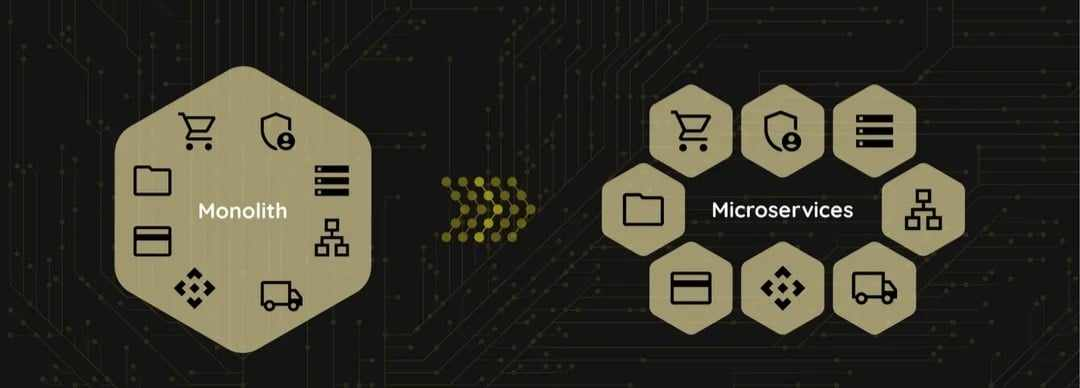
\includegraphics[height = 3cm]{pictures/ChuyenTu_KienTrucNguyenKhoi_Sang_KienTrucViDichVu.jpg}
% \caption{ViDuHinhAnhTheoChieuDoc}
\end{figure}

\begin{figure}[h]
\centering
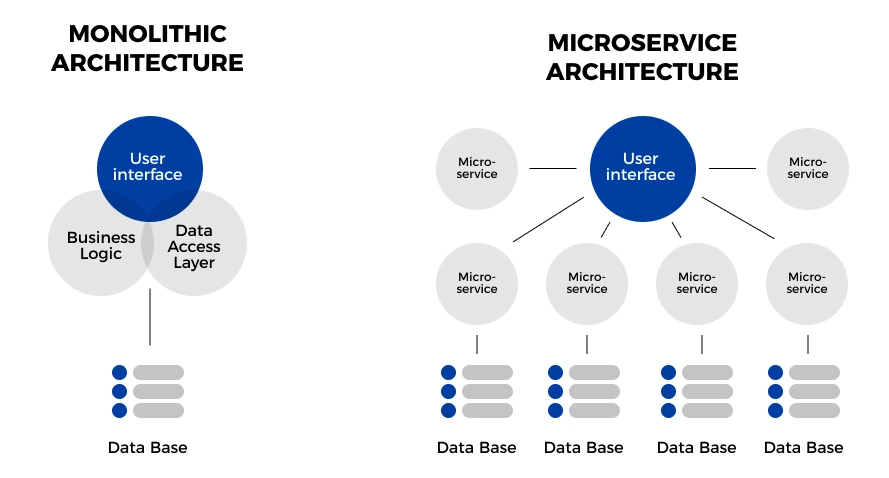
\includegraphics[height = 3cm]{pictures/AnhKhacNhau_KienTrucNguyenKhoi_KienTrucViDichVu.png}
% \caption{ViDuHinhAnhTheoChieuDoc}
\end{figure}

% Strangler Fig là chuyển mono sang dịch vụ

% kiến trúc vi dịch vụ Architecture : https:// thiết kế hướng miền - practitioners.com/?page_id = 398
% kiến trúc vi dịch vụ Architecture : https:// thiết kế hướng miền - practitioners.com/?page_id = 398
% kiến trúc vi dịch vụ Architecture : https:// thiết kế hướng miền - practitioners.com/?page_id = 398
% kiến trúc vi dịch vụ Architecture : https:// thiết kế hướng miền - practitioners.com/?page_id = 398
% kiến trúc vi dịch vụ Architecture : https:// thiết kế hướng miền - practitioners.com/?page_id = 398
% kiến trúc vi dịch vụ Architecture : https:// thiết kế hướng miền - practitioners.com/?page_id = 398
% kiến trúc vi dịch vụ Architecture : https:// thiết kế hướng miền - practitioners.com/?page_id = 398
% kiến trúc vi dịch vụ Architecture : https:// thiết kế hướng miền - practitioners.com/?page_id = 398
% kiến trúc vi dịch vụ Architecture : https:// thiết kế hướng miền - practitioners.com/?page_id = 398
% kiến trúc vi dịch vụ Architecture : https:// thiết kế hướng miền - practitioners.com/?page_id = 398

Trang chủTrang chủBảng chú giảiKiến trúc vi dịch vụ
Kiến trúc vi dịch vụ
Kiến trúc kiến trúc vi dịch vụ (hay đơn giản là kiến trúc vi dịch vụ) là một cách xây dựng các ứng dụng phần mềm dưới dạng tập hợp các dịch vụ nhỏ, độc lập giao tiếp với nhau thông qua API. Mỗi dịch vụ tập trung vào một khả năng kinh doanh cụ thể và có thể được triển khai, mở rộng quy mô và duy trì độc lập với các dịch vụ khác trong hệ thống. Cách tiếp cận này nhấn mạnh tính mô - đun, tính linh hoạt và khả năng phục hồi, cho phép các nhóm làm việc đồng thời trên các phần khác nhau của hệ thống và cho phép phát hành nhanh hơn và thường xuyên hơn. Các vi dịch vụ thường dựa vào các giao thức truyền thông nhẹ, chẳng hạn như REST và thường được triển khai bằng các công nghệ chứa trong bộ chứa như Docker và Kubernetes.

Đặc trưng
Dưới đây là một số đặc điểm của một kiến trúc kiến trúc vi dịch vụ tốt:

Mô - đun hóa : Kiến trúc nên bao gồm một tập hợp các dịch vụ được kết hợp lỏng lẻo có thể được triển khai, duy trì và mở rộng quy mô một cách độc lập.
Triển khai độc lập : Mỗi dịch vụ phải có khả năng triển khai độc lập để có thể thực hiện các thay đổi đối với một dịch vụ mà không ảnh hưởng đến các dịch vụ khác.
Bối cảnh giới hạn : Kiến trúc phải được thiết kế để phù hợp với ranh giới của khả năng kinh doanh, sao cho mỗi dịch vụ chịu trách nhiệm về một tập hợp chức năng cụ thể, gắn kết.
Tự chủ : Các dịch vụ phải có khả năng hoạt động tự chủ, ít phụ thuộc vào các dịch vụ khác.
Khả năng phục hồi : Kiến trúc phải được thiết kế để chịu đựng lỗi và các dịch vụ phải có khả năng xử lý lỗi một cách duyên dáng.
Khả năng mở rộng : Kiến trúc phải được thiết kế để hỗ trợ mở rộng quy mô các dịch vụ riêng lẻ cũng như toàn bộ hệ thống.
Tính linh hoạt : Kiến trúc phải cho phép phát triển và triển khai nhanh chóng các dịch vụ mới cũng như khả năng thay đổi các dịch vụ hiện có một cách nhanh chóng và dễ dàng.
Văn hóa DevOps : Kiến trúc phải được hỗ trợ bởi văn hóa nhấn mạnh sự cộng tác và giao tiếp giữa các nhóm phát triển và vận hành, cũng như tự động hóa các quy trình triển khai và thử nghiệm.
Nhược điểm
Mặc dù kiến trúc vi dịch vụ có nhiều lợi ích nhưng cũng có một số nhược điểm cần xem xét:

Độ phức tạp ngày càng tăng : Kiến trúc kiến trúc vi dịch vụ phức tạp hơn kiến trúc nguyên khối. Bản chất phân tán của kiến trúc vi dịch vụ khiến việc phát triển, thử nghiệm, triển khai và giám sát hệ thống trở nên khó khăn hơn.
Những thách thức về điện toán phân tán : Với kiến trúc vi dịch vụ, các dịch vụ khác nhau có thể chạy trên các máy khác nhau, khiến việc duy trì liên lạc giữa chúng trở nên khó khăn. Điều này có thể dẫn đến các vấn đề về độ trễ, tính nhất quán của dữ liệu và độ tin cậy.
Chi phí hoạt động : Với kiến trúc kiến trúc vi dịch vụ, có nhiều dịch vụ cần triển khai và quản lý, điều này có thể dẫn đến tăng chi phí hoạt động.
Ranh giới dịch vụ : Việc xác định ranh giới dịch vụ có thể là một thách thức, đặc biệt là trong các hệ thống phức tạp. Nếu không được thiết kế chính xác, điều này có thể dẫn đến sự phụ thuộc vào dịch vụ khiến việc thay đổi một dịch vụ trở nên khó khăn hơn.
Thách thức về tích hợp : kiến trúc vi dịch vụ thường yêu cầu tích hợp với các dịch vụ khác, điều này có thể khó đạt được. Các dịch vụ có thể có các giao thức, định dạng dữ liệu và phương thức liên lạc khác nhau, điều này có thể gây khó khăn cho việc tích hợp.
Chi phí chung của cổng API : Cần có cổng API để quản lý các API dịch vụ khác nhau và cung cấp giao diện hợp nhất cho khách hàng. Điều này có thể bổ sung thêm chi phí cho hệ thống.
Gỡ lỗi và kiểm tra: Việc gỡ lỗi và kiểm tra có thể phức tạp hơn trong kiến trúc kiến trúc vi dịch vụ do tính chất phân tán của hệ thống.
Nhìn chung, những nhược điểm của kiến trúc kiến trúc vi dịch vụ có thể được giảm thiểu bằng các phương pháp thiết kế và phát triển tốt. Tuy nhiên, điều quan trọng là phải cân nhắc giữa lợi ích và nhược điểm khi quyết định có nên sử dụng kiến trúc kiến trúc vi dịch vụ hay không.

thiết kế hướng miền có thể trợ giúp như thế nào
Thiết kế hướng miền (thiết kế hướng miền) có thể hỗ trợ kiến trúc và thiết kế kiến trúc vi dịch vụ theo nhiều cách:

Bối cảnh giới hạn : thiết kế hướng miền nhấn mạnh việc xác định các bối cảnh giới hạn, là các khu vực riêng biệt của miền có ranh giới được xác định rõ ràng. Điều này có thể giúp xác định ranh giới của kiến trúc vi dịch vụ và đảm bảo rằng mỗi kiến trúc vi dịch vụ đều có trách nhiệm rõ ràng và tập trung.
ngôn ngữ chung : thiết kế hướng miền khuyến khích sử dụng một ngôn ngữ chung được chia sẻ bởi cả chuyên gia ngành và nhân viên kỹ thuật. Điều này có thể giúp đảm bảo rằng các vi dịch vụ giao tiếp hiệu quả với nhau và phù hợp với yêu cầu kinh doanh.
Ánh xạ bối cảnh: thiết kế hướng miền cung cấp các kỹ thuật để ánh xạ các mối quan hệ giữa các bối cảnh giới hạn. Điều này có thể giúp đảm bảo rằng các vi dịch vụ được thiết kế với sự hiểu biết rõ ràng về sự phụ thuộc của chúng vào các dịch vụ khác.
Tập hợp: thiết kế hướng miền định nghĩa tập hợp là các cụm đối tượng liên quan cần được coi là một đơn vị nhất quán duy nhất. Điều này có thể giúp đảm bảo rằng các vi dịch vụ được thiết kế với sự hiểu biết rõ ràng về các yêu cầu về tính nhất quán của dữ liệu.
Tương quan với bối cảnh giới hạn
Mặc dù người ta thường khuyên nên căn chỉnh ranh giới của kiến trúc vi dịch vụ với ranh giới của bối cảnh giới hạn, nhưng điều đó không phải lúc nào cũng cần thiết hoặc khả thi. Một vi dịch vụ có thể gói gọn nhiều ngữ cảnh giới hạn hoặc một ngữ cảnh giới hạn có thể được phân chia thành nhiều vi dịch vụ, tùy thuộc vào nhu cầu cụ thể của hệ thống và sự cân bằng liên quan. Cuối cùng, mục tiêu là tạo ra một hệ thống mô - đun và có thể bảo trì, đáp ứng các yêu cầu kinh doanh và mối quan hệ giữa bối cảnh giới hạn và các vi dịch vụ phải được thiết kế phù hợp.

Tương quan với API thực thể
Nhìn chung, việc thiết kế các vi dịch vụ chỉ dựa trên các hoạt động CRUD của thực thể không được khuyến khích vì nó có thể dẫn đến một kiến trúc liên kết chặt chẽ và không hiệu quả. Các vi dịch vụ phải được thiết kế dựa trên khả năng kinh doanh, có thể phù hợp hoặc không phù hợp với hoạt động CRUD của thực thể.

thiết kế hướng miền có thể giúp xác định các khả năng kinh doanh và xác định bối cảnh giới hạn, sau đó có thể được sử dụng để hướng dẫn thiết kế các vi dịch vụ. Bằng cách tập trung vào khả năng kinh doanh thay vì hoạt động CRUD thực thể, các vi dịch vụ có thể được liên kết lỏng lẻo hơn, mang tính mô - đun hơn, dễ dàng duy trì và phát triển hơn theo thời gian.

Tương quan với SOA (Kiến trúc hướng dịch vụ)
Kiến trúc kiến trúc vi dịch vụ là sự phát triển của mô hình kiến trúc hướng dịch vụ (SOA), trong đó nhấn mạnh đến các dịch vụ có khả năng tương tác và liên kết lỏng lẻo. Tuy nhiên, kiến trúc kiến trúc vi dịch vụ khác với SOA ở một số điểm chính.

Đầu tiên, các vi dịch vụ thường nhỏ hơn và tập trung hơn vào các khả năng kinh doanh cụ thể so với các dịch vụ trong SOA truyền thống. Điều này làm cho chúng dễ dàng phát triển, thử nghiệm và bảo trì hơn cũng như có khả năng phục hồi tốt hơn trước sự thay đổi.

Thứ hai, các vi dịch vụ có xu hướng phụ thuộc nhiều hơn vào các giao thức truyền thông và định dạng dữ liệu nhẹ, chẳng hạn như REST và JSON, trong khi SOA thường sử dụng các giao thức nặng hơn như SOAP và XML.

Cuối cùng, các vi dịch vụ thường chú trọng nhiều hơn đến các nhóm tự chủ và việc ra quyết định phi tập trung hơn so với SOA, vốn có thể có khả năng quản trị và kiểm soát tập trung hơn.

Nhìn chung, mặc dù có một số điểm trùng lặp giữa hai kiến trúc, nhưng kiến trúc vi dịch vụ thể hiện một cách tiếp cận hiện đại, linh hoạt hơn đối với thiết kế phần mềm dựa trên dịch vụ.

